\subsection{Explicación formal del problema}

Sea una matriz $M$ $\in$ $\mathbb{R}^{n \times m}$, donde cada posición de la matriz $M_{ij}$ tiene un valor asociado $h_{ij}$. El problema consiste en calcular el camino mínimo de casilleros desde la posición (1,1) hasta la posición ($N$,$M$), donde los únicos dos  movimientos posibles son:

\emph{Moverse hacia el casillero superior}: \[M_{i,j} \rightarrow M_{i+1,j}\] 

ó \emph{Moverse hacia el casillero de la derecha}: \[M_{i,j} \rightarrow M_{i,j+1}\]

Realizar estos movimientos tiene un costo que depende de un parámetro de entrada $H$:

\begin{equation} \label{costoHaciaArriba}
   Costo(M_{i,j} \rightarrow M_{i+1,j}) = \left\{ 
     \begin{array}{lr}
       0 							& $ si $  |h_{i,j} - h_{i+1,j}| \leq H \\
       |h_{i,j} - h_{i+1,j}| - H 	&   $ caso contrario $ \\
     \end{array}
   \right.
\end{equation} 

\begin{equation}\label{costoHaciaDerecha}
  Costo(M_{i,j} \rightarrow M_{i,j+1}) = \left\{ 
     \begin{array}{lr}
       0 							& $ si $  |h_{i,j} - h_{i,j+1}| \leq H \\
       |h_{i,j} - h_{i,j+1}| - H 	&   $ caso contrario $ \\
     \end{array}
   \right.
\end{equation} 

%\subsubsection{Modelado del problema con grafos}
%
%Para resolver el problema vamos a modelar la matriz $M$ $\in$ $\mathbb{R}^{n \times m}$ con un grafo dirigido $G=(V,E)$, donde $V$ es el conjunto de nodos y $E$ el conjunto de aristas (orientadas) del grafo. Cada nodo $v_{i,j} \in V$ representa a una posición de la matriz $(i,j)$, y las aristas representarán los posibles movimientos entre dos nodos dentro de la matriz (\emph{Moverse hacia el casillero superior} y \emph{Moverse hacia el casillero de la derecha}). Es decir, 
%
%\begin{align*}
%(\forall i,i\prime \in [1..n],\ j,j\prime \in [1..m]) \ : & \\ 
%(v_{i,j}, v_{i\prime, j\prime}) \in E \hfill \ \ \ \Leftrightarrow \hfill \ \ \
%& (i\prime, j\prime) = (i+1,j) \\
%o\ & (i\prime, j\prime) = (i,j+1) \\
%\end{align*}
%
%Además, definimos $\kappa : E \rightarrow \mathbb{R}$ el peso de las aristas, como el costo que implica realizar dichos movimientos (dado por las funciones \ref{costoHaciaArriba} y \ref{costoHaciaDerecha}):
%\begin{equation}
%\kappa (v_{i,j}, v_{i\prime, j\prime}) = Costo (M_{i,j} \rightarrow M_{i\prime, j\prime})
%\end{equation}
% 
%Modelando el problema de esta manera, el problema se traduce en encontrar el camino mínimo (el camino de menor costo entre todas las aristas) en $G$ desde el vértice $v_{1,1}$ hasta el vértice $v_{n,m}$. 

\subsubsection{Ejemplos}

% Ejemplo de una matriz, y la solucion del camino. A TERMINAR

\subsection{Formulación Recursiva}

Obtendremos la solución del problema usando un algoritmo de programación dinámica. Para eso, planteamos una formulación recursiva del problema. Sea la función $f$:

$f(i,j) = $ costo de un camino óptimo desde $ M_{1,1} $ hasta $ M{i,j}$

Entonces, la solución del problema está dada por $f(n,m)$. 
Se propone la siguiente recursión para calcular $f$:

\begin{equation} \label{formulacionRecursiva}
f(i,j) = min \left( 
	\begin{array}{lr}
    f(i-1, j) + Costo(M_{i-1,j} \rightarrow M_{i,j}), \\
	f(i,j-1) + Costo(M_{i,j-1} \rightarrow M_{i,j}) \\
     \end{array}
   \right)
\end{equation}  

con algunos casos particulares:

$f(1,1) = 0 $

$f(1,j) = f(1,j-1) + Costo(M_{1,j-1} \rightarrow M_{1,j})$

$f(i,1) = f(i-1,1) + Costo(M_{i-1,1} \rightarrow M_{i,1})$

\subsubsection{Demostración de Correctitud}

El caso base $f(1,1)$ es trivial, ya que no realizo ningún movimiento.

Dada cualquier otra posición $(i,j)$ de la matriz, el camino mínimo para llegar a ella tiene como última posición visitada o la casilla de su izquierda $(i, j-1)$ (si existe), o la casilla de abajo $(i-1, j)$ (si existe) por el enunciado del problema, ya que los únicos movimientos posibles son moverse hacia arriba o hacia la derecha.

Para demostrar que la función $f$ propuesta calcula el camino mínimo hasta la casilla cualquiera $M_{i,j}$ debemos ver que se cumple el \textbf{Principio de Optimalidad.} Es decir, que dado un camino óptimo desde $M_{1,1}$ hasta $M{i,j}$, $P_{i,j}$, entonces, el subcamino desde $M_{1,1}$ hasta el inmediato antecesor de $M_{i,j}$ ($P_{i-1,j}$ o $P{i,j-1}$) debe ser óptimo: 

Sea $P_{i,j}$ el camino óptimo desde $M_{1,1}$ $hasta M{i,j}$.
SPGE, puedo suponer que el inmediato antecesor de $M_{i,j}$ en $P$ es $M_{i, j-1}$. Supongamos que elsub camino hasta el antecesor de $M_{i,j}$ ($P_{i,j-1}$)  no es óptimo. Entonces, $\exists$ $P\prime_{i,j-1}$ tal que $Costo(P\prime_{i,j-1})$ $<$ $Costo(P_{i,j-1})$.

Pero entonces, puedo tomar el camino  $P\prime_{i,j-1}$ y de ahí moverme a la posición $M_{i,j}$. 
$Costo (P\prime_{i,j-1}) + Costo(M_{i-1,j} \rightarrow M_{i,j}) < Costo (P{i,j-1}) + Costo(M_{i-1,j} \rightarrow M_{i,j}) = Costo(P_{i,j})$
Pero esto es absurdo, ya que existiría un camino mejor que el óptimo hasta la posición $(i,j)$.

Como aplica el principio de optimalidad y sólo hay dos posibles antecesores para una determinada casilla $M_{i,j}$, para calcular el camino mínimo hasta una posición $(i,j)$ basta con tomar el mínimo entre las dos posibilidades, tomando el cuenta el costo de realizar el último movimiento.

Para los casos borde de la matriz, en la primera columna y en la primera fila, donde sólo tengo un sólo posible antecesor (el inmediato de abajo y el inmediato de la izquierda respectivamente), el camino mínimo entonces es el camino mínimo hasta el único antecesor más el último movimiento. $\qed$

\subsection{Pseudocódigo}

% Explicacion del pseudocodigo, y de cómo se guarda el camino
% Representacion del diccionario

\subsubsection{Enfoque top-down vs. bottom-up}

% Dependencias, algoritmo iterativo...

\subsection{Complejidad del algoritmo}

\subsubsection{Complejidad en peor caso}

\subsubsection{Complejidad en mejor caso}

\subsection{Performance del algoritmo}


Como dijimos antes, la complejidad del algoritmo es siempre $\Theta(n m)$, sin distinción entre casos, por lo que el análisis de performance es simple.

Primero veamos que, en la práctica, la complejidad del algoritmo es efectivamente $\Theta(n \log n)$.

\begin{figure}[H]
 \centering
	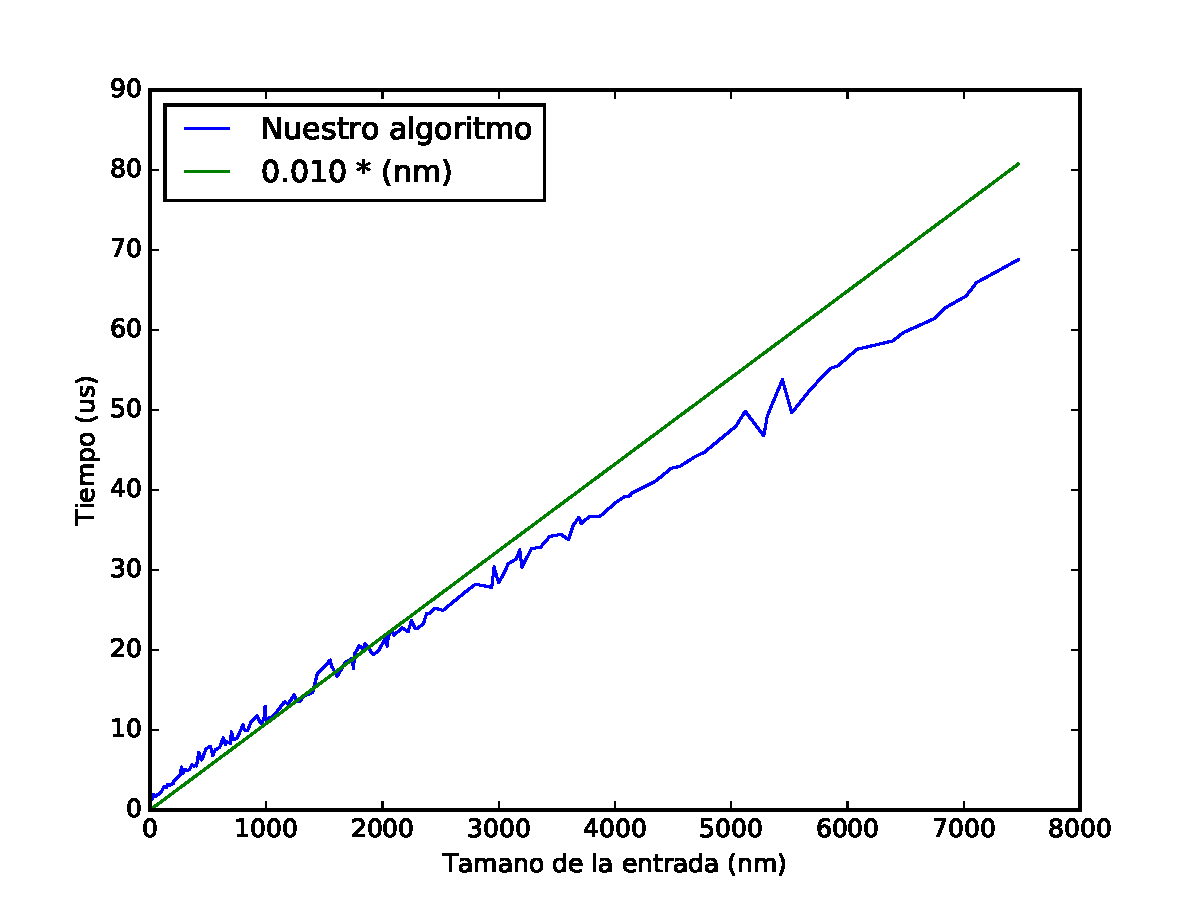
\includegraphics[width=0.8\textwidth]{img/exp/problema3-promedio.pdf}
	\caption{\footnotesize Tiempo que toma el algoritmo en $\mu$s para una entrada de tamaño $mn$.}
	\label{fig:problema3-promedio}
\end{figure}

En esta imagen se ve que se comporta como debe. Sin embargo, al igual que en los problemas anteriores, para confirmarlo totalmente, realizamos el gráfico de $\frac{T(nm)}{nm}$, dado que si esta función tiene a una constante cuando $nm \to \infty$, habremos confirmado experimentalmente que la complejidad del algoritmo es de $\Theta(n m)$.

\begin{figure}[H]
 \centering
	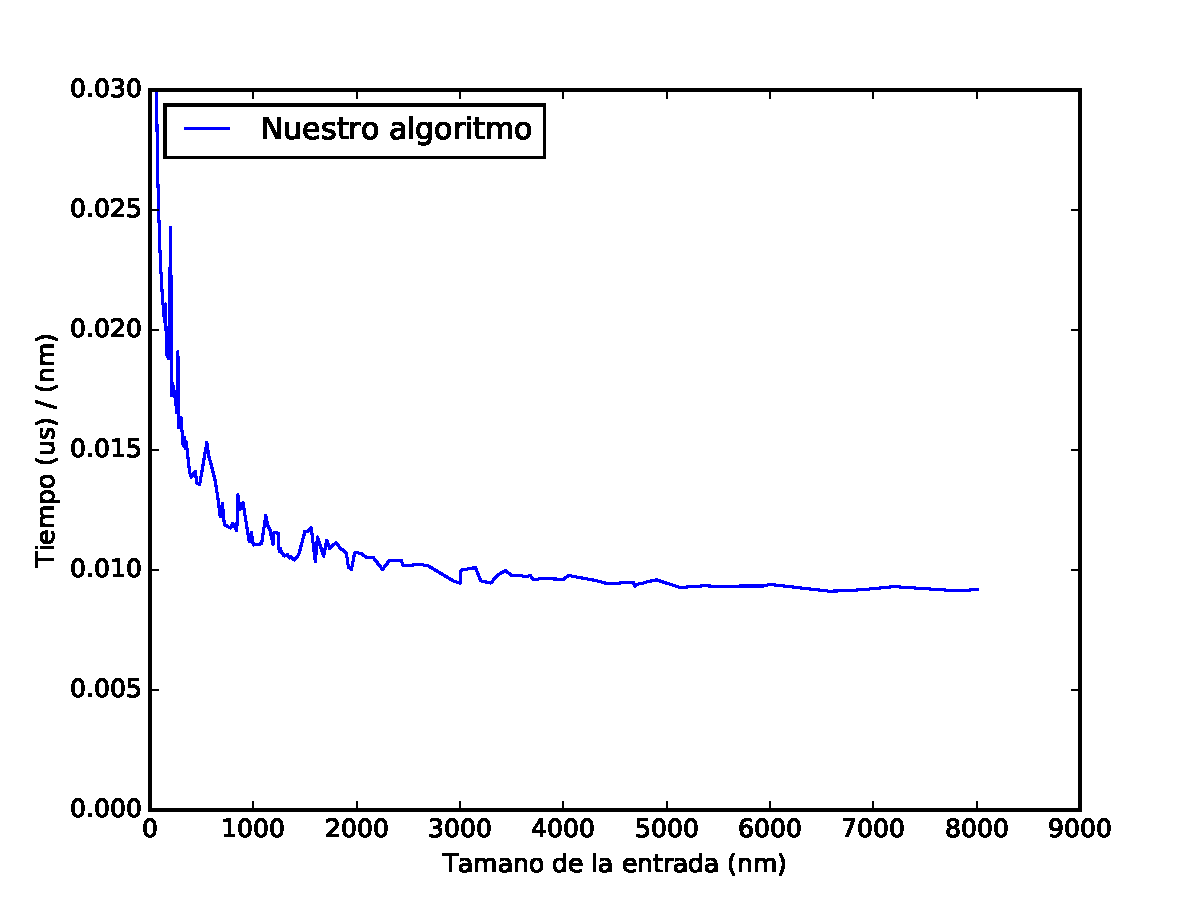
\includegraphics[width=0.8\textwidth]{img/exp/problema3-promedio2.pdf}
	\caption{\footnotesize Tiempo que toma el algoritmo en $\mu$s dividido $mn$ para una entrada de tamaño $mn$.}
	\label{fig:problema3-promedio2}
\end{figure}


\subsubsection{M\'etodo de experimentación}

